\documentclass[12pt]{article}
\usepackage[margin=1.0in]{geometry}
\usepackage[utf8]{inputenc}
\usepackage[T1]{fontenc}
\usepackage{lmodern}
\usepackage[spanish]{babel}
\usepackage{amsmath}
\usepackage{graphicx}
\usepackage{multicol}

\title{Sombrero Galaxy (M104) Rotation curve }

\begin{document}

\maketitle

\author{Wesley Peters $\&$ Juan Nicolas Garavito-Camargo}

Advisor: Jacqueline van Gorkom.

\section{Introduction}

HI observations are an useful tool to study galaxy rotation
curves. Observing  the shift in the wavelength of the 21cm line, we
can deduce that the part of the galaxy moving toward us would present
a blueshift while the part moving away us would present a
redshift. Observations at different distances from the galactic center
will let us construct the rotation curve of the galaxy. For our line of
sight, M104 is edge-on, effectively eliminating inclination
corrections. In this project we construct the rotation curve of the
Sombrero Galaxy (M104) from HI observations provided by Jacqueline van Gorkom.

\section{Methods}

\subsection{P/V diagram}

In the CASA Viewer, it is quite simple to obtain a Position/Velocity (P/V)
diagram. By selecting the P/V tool in the menu bar, one can highlight
a region and generate the diagram. The P/V diagram depends greatly on
the individual parameters of the galaxy, such as inclination or gas
distribution. Thankfully, CASA takes care of all of this and outputs
the radial velocity as a function of offset in arcseconds. This
diagram is shown in Figure 1. 

\begin{figure}
\begin{center}
\includegraphics[scale=0.25]{pv.png}
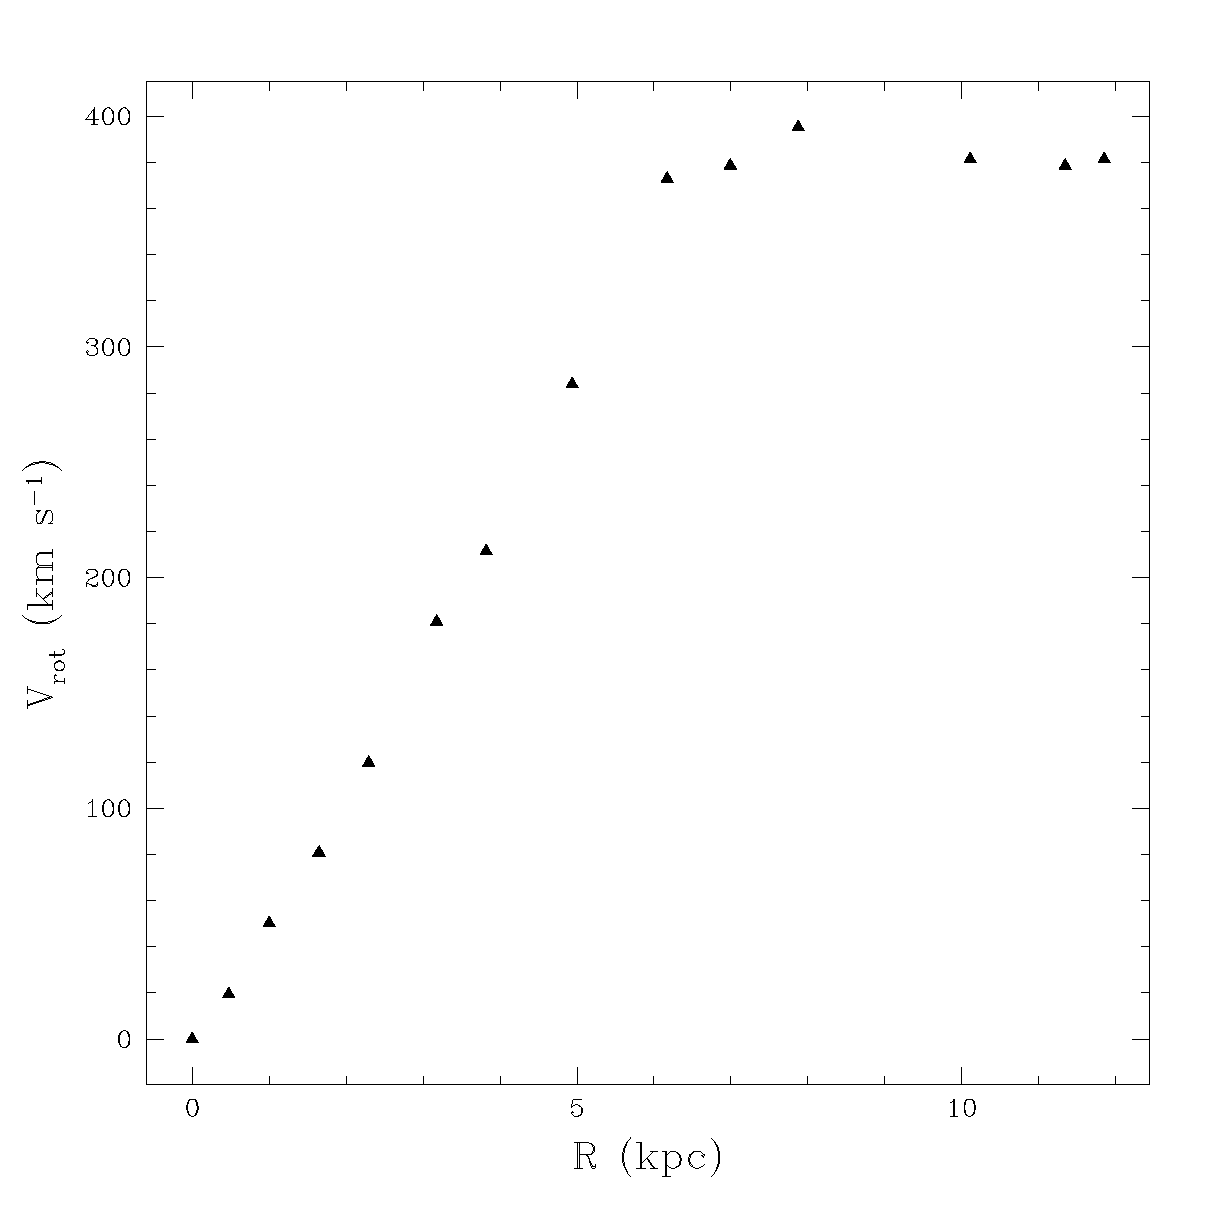
\includegraphics[scale=0.3]{rotcrv.eps}
\caption{(\textbf{Left})P/V Diagram of M104. (\textbf{Right})Rotation Curve of the Sombrero Galaxy (M104)}
\end{center}
\end{figure}



\subsection{Rotation Curve}

The rotation curve extracted from the P/V diagram is shown in Figure
2. In order to display the rotation curve as a function of physical
units, kiloparsecs, we used the small angle approximation:

\begin{equation}
kpc = D(0.000004848)\theta
\end{equation}
where D is the distance in kiloparsecs and $\theta$ is the angular size
of the object. We simply used the distance given by the $\emph{NASA/IPAC
Extragalactic Database}$ (NED), 10.35 Mpc. The proper method of
determining the rotation curve, fitting contours, was simplified by
reading off the rotation curve by eye.

The rotation curve of M104 exhibits a very fast rise, common of bulge
dominated galaxies. The rotation curve also flattens out around 380
km/s at $\sim$ 6 kpc from the center. 

\section{Discussion}

\subsection{Morphology of M104}

The most striking feature of M104 is its very large bulge, hence the
nickname ``Sombrero''. The effect of this bulge is seen in the
rotation curve via the steep, linearly rising component of the
rotation curve in the inner radii of the galaxy. Due to this large
bulge, the majority of this galaxy's gas and star formation is
relegated to a ring around the center, clearly visible in the r-band
image provided by Jacqueline van Gorkom.

\subsection{Mas}

In order to obtain the mass of the galaxy we assume that the system 
is in equilibrium i.e:
\begin{equation}
2T = U
\end{equation}

This lets us compute the velocity terms of the mass of the galaxy, and the radii.

\begin{equation}
mv^{2} = \dfrac{GMm}{r}
\end{equation}

\begin{equation}
v = \sqrt{\dfrac{GM}{r}}
\end{equation}

From the rotation curve Figure. we take a radii of $r = 12 kpc$ with a corresponding
velocity of $v=380 km\ s^{-1}$ and also with the gravity constant in units of pc and
$M_{\odot}$ $G = 4.302\times 10^{-3} \dfrac{pc}{M_{\odot}} (\dfrac{km}{s})^{2}$ we obtain 
a mass of:\\
 
\begin{equation}
M = \dfrac{rv^{2}}{G} = 4.699\times 10^{11} M_{\odot}
\end{equation}

This mass is in agreement with previous works which reports that M104 is $ \sim 4 M_{MW}$
the mass of the Milky Way, and its contribution is mainly due 
to the barionic matter, due to the fact that we are working for radius $r < 14Kpc$
we don't see a strong contribution of the dark matter halo. 


\end{document}



